\documentclass[dvipdfmx,titlepage]{jsarticle}
\usepackage[dvipdfmx]{graphicx}
\usepackage{bm}
\usepackage{amsmath}
\usepackage{amssymb}
\usepackage{amsfonts}
\usepackage{cases}
\usepackage{here}
\usepackage{capt-of}
\usepackage{multirow}
\usepackage{comment}
\usepackage{listings}
\usepackage{amsmath}
\usepackage{cases}
\usepackage{fancyvrb}
\usepackage{listings}
\usepackage{comment}
\usepackage{pdfpages}
\usepackage{siunitx}
\lstset{
    basicstyle={\ttfamily},
    identifierstyle={\small},
    commentstyle={\small\itshape},
    keywordstyle={\small\bfseries},
    ndkeywordstyle={\small},
    stringstyle={\small\ttfamily},
    frame={tb},
    breaklines=true,
    columns=[l]{fullflexible},
    numbers=left,
    xrightmargin=0zw,
    xleftmargin=3zw,
    numberstyle={\scriptsize},
    stepnumber=1,
    numbersep=1zw,
    lineskip=-0.5ex,
    keepspaces=true,
    language=c++
}
\renewcommand{\lstlistingname}{リスト}
\makeatletter
\newcommand{\figcaption}[1]{\def\@captype{figure}\caption{#1}}
\newcommand{\tblcaption}[1]{\def\@captype{table}\caption{#1}}
\makeatother
\fvset{
  fontsize=\small,%  フォントサイズをsmallに
  frame=single,%     枠で囲う (lines でもよいかも)
  numbers=left,%     左に行番号を付ける
  tabsize=4,%        タブは半角4文字分に変換
  baselinestretch=0.8%  行送りを標準の0.8倍に詰める
}
\newcommand{\Figref}[1]{\figurename~\ref{#1}}
\newcommand{\Tblref}[1]{\tablename~\ref{#1}}

\title{\Huge{数値解析レポートNo.4}}
\author{\huge{43番 若月 耕紀}}
\date{}

\begin{document}
\maketitle
\newpage


\section{以下を充たす$(x, y)$を$t = [0, 2]$の範囲で求めよ.\protect\linebreak
$\dfrac{dx}{dt} = x + 6y + t - 10, \:\:\:x(0) = 1\raisebox{4ex}{\mbox{}}$\protect\linebreak
$\dfrac{dy}{dt} = x + t - 3, \:\:\:y(0) = 2\raisebox{4ex}{\mbox{}}$}
\:

まず,理論値を求める.上式の理論値は以下のようになる.
\begin{eqnarray}
x &=& -2\exp(-2t)-t+3 \nonumber \\
y &=& \exp(-2t)+1 \nonumber
\end{eqnarray}

与式を,
\begin{eqnarray}
f(x, y; t) &=& \frac{dx}{dt} = x + 6y + t - 10 \nonumber \\
g(x, y; t) &=& \frac{dy}{dt} = x + t - 3 \nonumber
\end{eqnarray}

と考えると,$x, y$の値をオイラー法のように解くことができる.以下に示す式を実装する.
\begin{eqnarray}
x_{i+1} = x_i + f(x_i, y_i; t)dt \nonumber \\
y_{i+1} = y_i + g(x_i, y_i; t)dt \nonumber
\end{eqnarray}

上記を基に連立微分方程式を解く関数をリスト1に示す.

\begin{lstlisting}[caption=d\_euler, label=c]
#define f(x, y, t) (x + (6 * y) + t - 10)
#define g(x, y, t) (x + t - 3)

void d_euler(double t, double dt, double tn, double x0, double y0){
	int i;
	double n;
	double *x, *y;

	//要素数
	n = (tn - t) / dt;

	//メモリ確保
	x = (double*)malloc(sizeof(double) * n);
	y = (double*)malloc(sizeof(double) * n);

	//初期値代入
	x[0] = x0;
	y[0] = y0;
	printf("%f, %f, %f\n",t , x[0], y[0]);

	//オイラー法
	for(i = 1; t <= tn; i++){
		x[i] = x[i - 1] + f(x[i - 1], y[i - 1], t) * dt;
		y[i] = y[i - 1] + g(x[i - 1], y[i - 1], t) * dt;
		t += dt;
		printf("%f, %f, %f\n",t , x[i], y[i]);
	}

	//メモリ解放
	free(x);
	free(y);
}
\end{lstlisting}

入力として$t$の初期値,ステップ幅$dt$,$t$の最終値,$x$の初期値,$y$の初期値の順で与え,オイラー法のように解く.

この関数を用いて求めた各要素数ごとの$x, y$の解と理論値を,図1, 2に示す.

\begin{figure}[h]
\begin{minipage}{0.5\hsize}
	\centering
	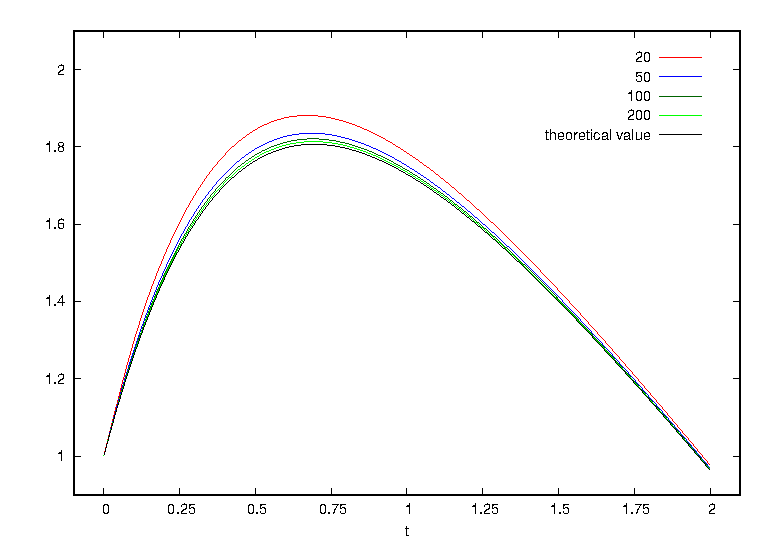
\includegraphics[width=8cm]{x.eps}
	\caption{$xの解$}
	\label{fig:4-1}
\end{minipage}
\begin{minipage}{0.5\hsize}
	\centering
	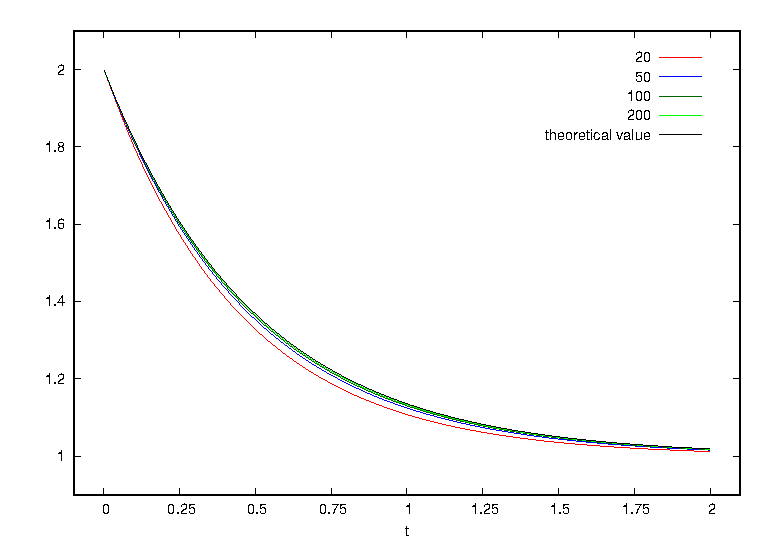
\includegraphics[width=8cm]{y.eps}
	\caption{$yの解$}
	\label{fig:4-2}
\end{minipage}
\label{fig:5}
\end{figure}

上記の結果より,要素数の増加,つまりステップ幅が狭いほど正確な値が求められることがわかる.

\section{$x = 1$における以下の微分方程式の解$y$を求めよ\protect\linebreak
$\dfrac{d^2y}{dx^2} + 5\dfrac{dy}{dx} - 6y = 0, \:\:\:y(0) = 0, \:\:\:\dfrac{dy}{dx}(0) = 7\raisebox{4ex}{\mbox{}}$}
\:

まず,理論値を求める.上式の理論値は,以下のようになる.
\begin{eqnarray}
y &=& \exp(x) - \exp(-6x) \nonumber\\
&\approx& 2.7158\:\:\:(x = 1)\nonumber
\end{eqnarray}

与式について,$\dfrac{dy}{dx} = z$を導入すると,
\begin{eqnarray}
\frac{dy}{dx} &=& z \nonumber \\
\frac{dz}{dx} &=& 6y - 5z \nonumber
\end{eqnarray}

となる.これは,独立変数$x$に関する連立微分方程式なので,第1節と同じ方法で解くことができる.

リスト1の関数を用いて求めた各要素ごとの$y$の解と,理論値を図3に示す.
\begin{figure}[htbp]
  \begin{center}
    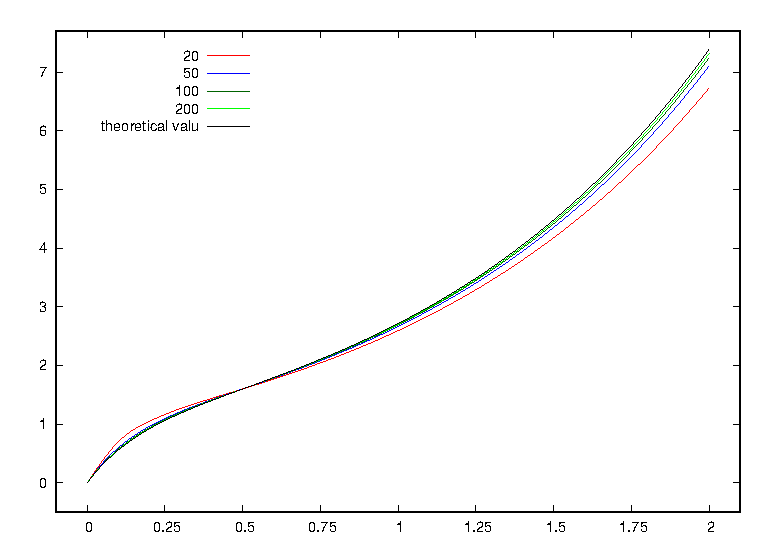
\includegraphics[width=8cm]{yy.eps}
    \caption{yの解}
    \label{q12}
  \end{center}
\end{figure}

この関数を用いて解析を行った結果,$x = 1$では$y = 2.702759$が出力された.これは,理論値である$y\approx 2.7158$とほぼ等しいことがわかる.

\section{感想}
今回のレポートは早めに始め,かつ期限に余裕をもって完成させることができた.これまでの課題を解決することができて良かった.また,今回のプログラムは課題で完成させていたものを少し変えるだけだったため,理解がしやすかった.これで最後のレポートとなったが,全てのレポートを提出することができて良かったと思う.


\end{document}